% Copyright (c) 2019-2020  Zubax Robotics  <info@zubax.com>
%
% Distributed under BY-NC-ND (attribution required, non-commercial use only, no derivatives).
%

\documentclass{document_templates/documentation_template_latex/zubaxdoc}
\graphicspath{{document_templates/documentation_template_latex/}{figures/}}
\title{Zubax Sadulli Datasheet}

\hbadness=10000

\begin{document}
\frontmatter
\begin{titlepage}

\section*{Overview}

Zubax Sadulli is a tightly integrated unit that contains a motor and its control electronics in a compact enclosure. 
Sadulli is a turn-key solution for propulsion systems for light unmanned aerial applications. 
It is based on \mbox{mitochondrik} control module. 
All hardware is open source and available on Github\footnote{\url{https://github.com/Zubax/sadulli}}.

\section*{Features}

\begin{itemize}
    \item 550 W continuous power output
    \item 12 -- 34 V input voltage range (4 -- 8S $\text{LiCoO}_\text{2}$ battery)
    \item Software controllable 5 V, 0.5 A BEC
    \item High-efficiency sensorless FOC algorithms
    \item Self-diagnostics and health status reporting
    \item Built-in motor temperature sensor for enhanced self-diagnostics
    \item Ready right out of the box, all parameters are pre-tuned for high dynamic response and high-efficiency operation
    \item Highly configurable, all parameters can be tuned
    \item Embedded bootloader. Firmware can be updated via CAN interface in the field, no need to unmount the unit.
    \item Regenerative braking and active freewheeling
    \item The solder-free design facilitates in-field maintenance
    \item Low noise and high efficiency due to the sinusoidal \mbox{motor} currents and high-frequency PWM
    \item UAVCAN support
\end{itemize}

\section*{Applications}

\begin{itemize}
    \item \mbox{Propeller drives for multirotor unmanned aerial vehicles}
\end{itemize}

\centering
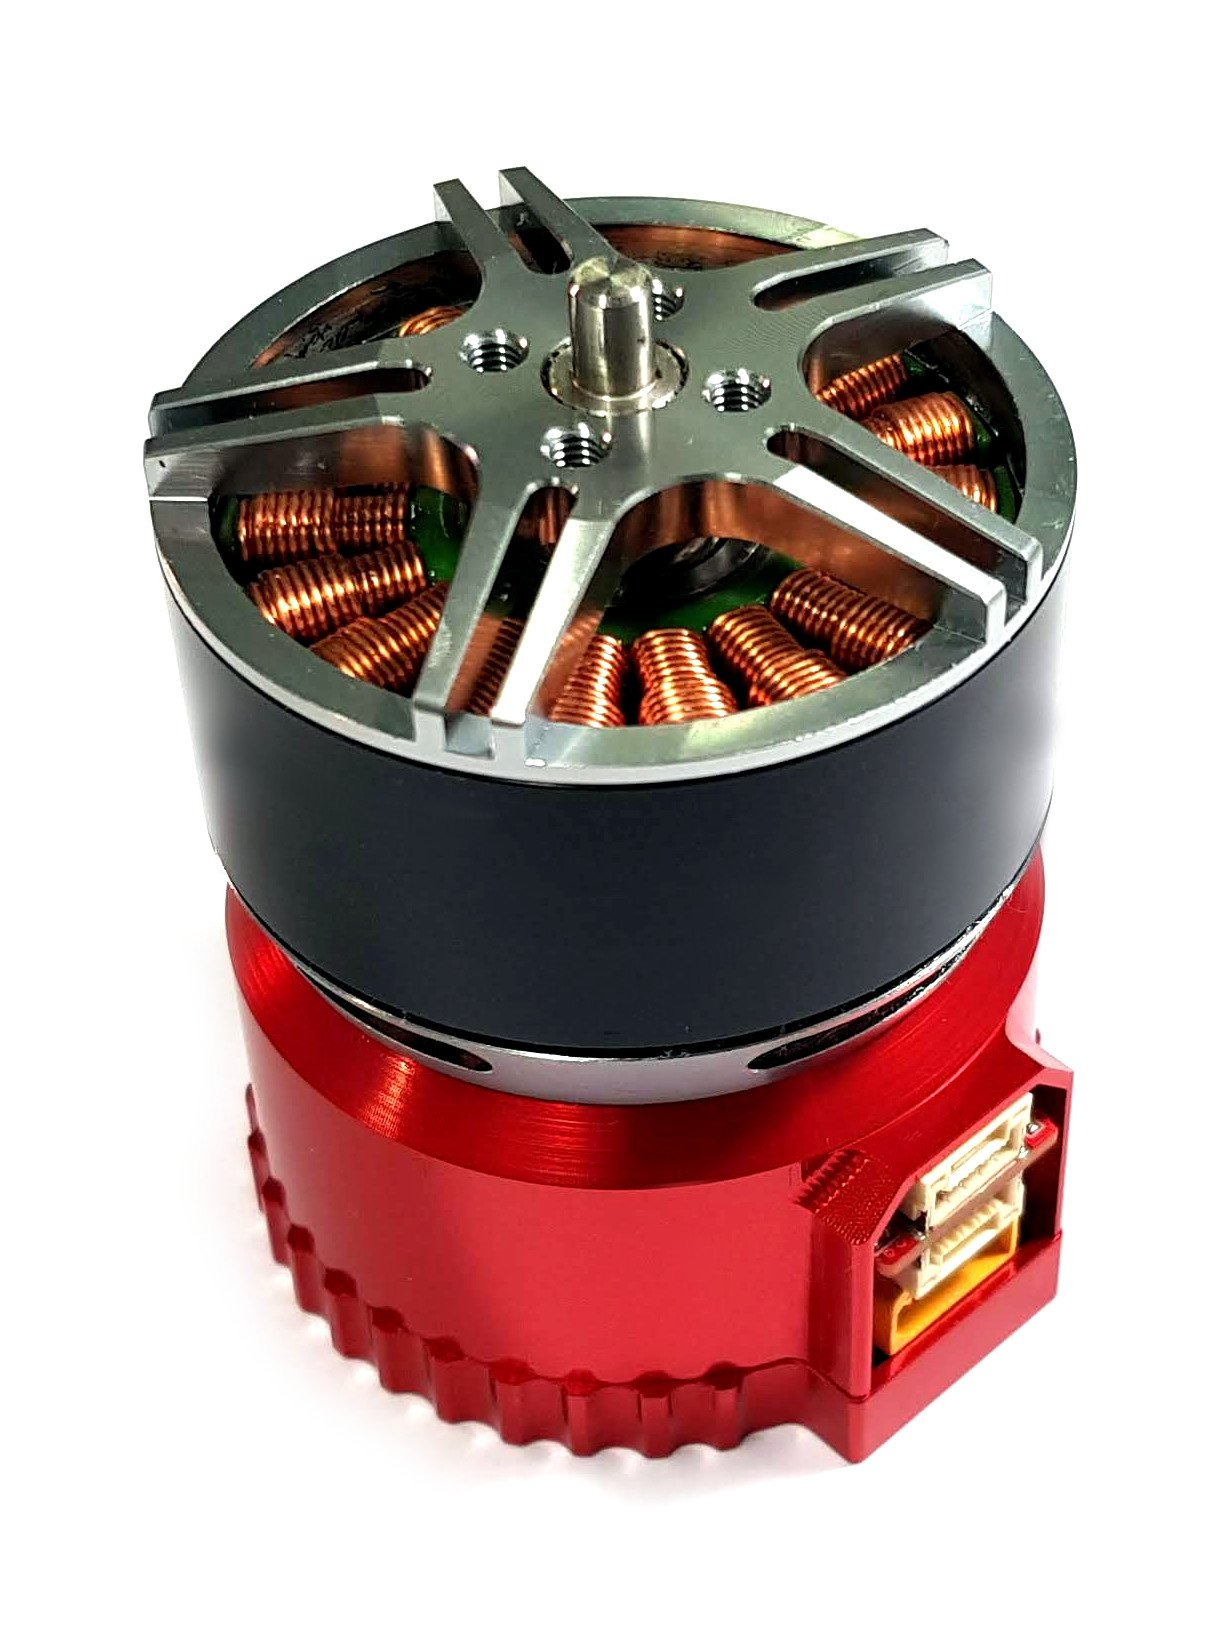
\includegraphics[width=0.42\textwidth]{sadulli_grosso_pic}
\end{titlepage}

\tableofcontents
\BeginRightColumn
\listoffigures
\listoftables

\mainmatter

\chapter{Overview}

Sadulli is a tightly integrated unit that contains an electric motor with a sensorless electronic speed controller 
in a single monolithic package. Sadulli supply package includes an integrated drive and a propeller. 
Sadulli comes pre-tuned for its particular motor and propeller, 
which ensures high-efficiency operation and excellent dynamic response. 
Compact and tightly integrated design minimizes motor wiring and hence internal resistance, which, in turn, 
means fewer power losses and EMI.
The controller provides up to 500 W of continuous power output and supports a wide range of operating voltages 
12-33.6 V (4–8S $\text{LiCoO}_\text{2}$ battery).

Although the device comes completely pre-tuned comprehensive fine-tuning is still available to the end-user.
Zubax Sadulli is fully UAVCAN compatible and enables easy integration into the end system by 
using a full set of standard UAVCAN Micro connectors
\footnote{For more details refer to \url{https://uavcan.org/Specification/8._Hardware_design_recommendations/}}.

Zubax Sadulli constantly measures and reports all the crucial variables during operation 
(like the controller’s temperature, motor temperature, current consumption, battery voltage, etc.) 
improving system reliability.

Zubax Sadulli is an open hardware reference design for Mitochondrik.
Mitochondrik is an integrated module (like an integrated circuit) that enables third-party hardware engineers 
to design sophisticated custom motor controllers using motor control technology – T\'elega, 
which integrates advanced control algorithms. This datasheet is focused only on the Sadulli Hardware.

\section{System integration}
Zubax Sadulli is a single supply device, which means that the device does not expose any power supply inputs 
except for the high power supply. The 5 V rails of the CAN interfaces are not used by the device; 
rather, the device may provide 5 V power line for UAVCAN bus from its internal DC-DC converter if needed.

\begin{figure}[h]
    \centering
    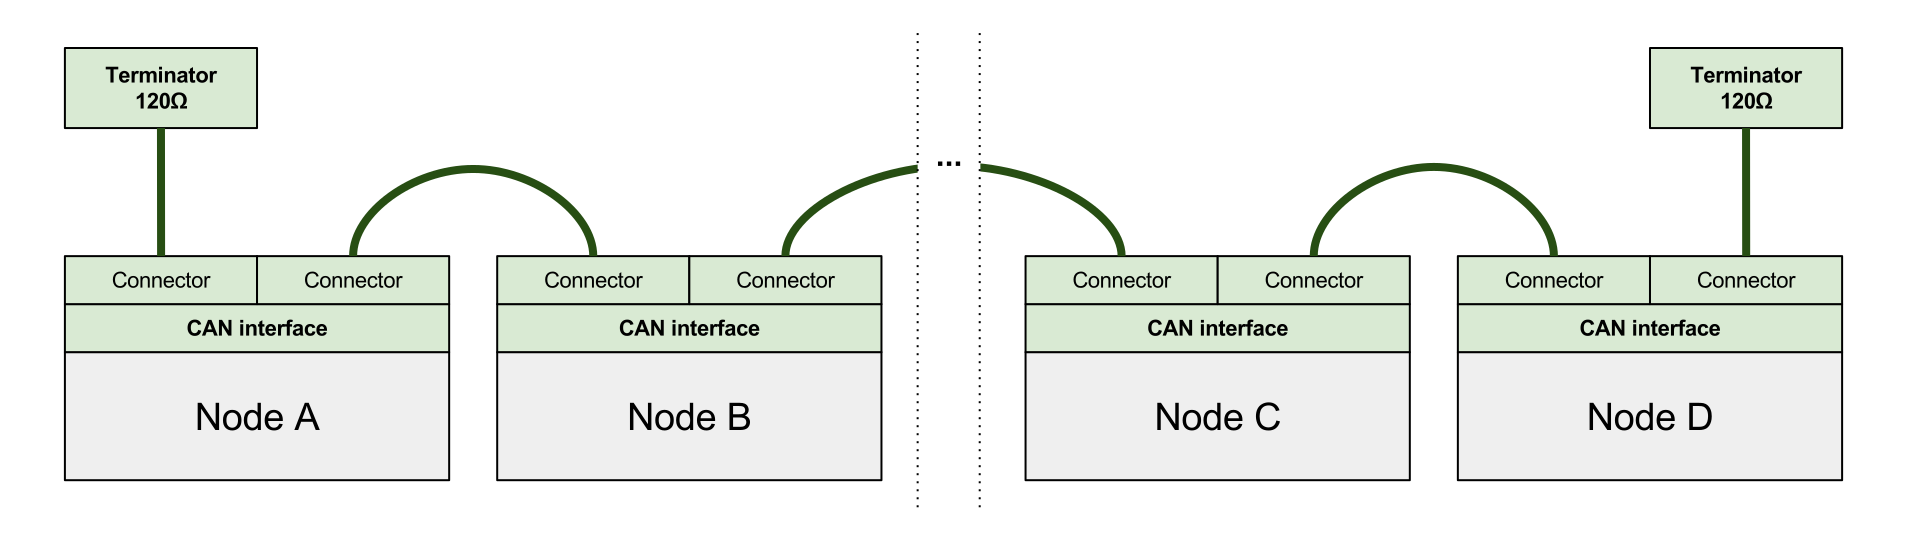
\includegraphics[width=1\textwidth]{figures/can_integration.png}
    \caption{Connection of CAN nodes}
\end{figure}

\section{Variants}

Three versions of Sadulli hardware are available:
\begin{itemize}
    \item \textbf{Sadulli Piccino} can be applied for light multirotor aircraft with takeoff mass up to 1500 g/rotor. 
    \item \textbf{Sadulli Grosso} can be applied for multirotor aircraft with takeoff mass 4000 g/rotor
    \item \textbf{Sadulli Nudo} is a version of the hardware that does not include the motor and propeller 
    and is supposed to be used with the vendor's motor of choice. It can also be fine-tuned for that motor if requested.
\end{itemize}

\begin{ZubaxTableWrapper}{Sadulli variants}
\begin{ZubaxWrappedTable}{| L | X | X |}\label{table:Sadulli variants}
    Version     & Motor     & Propeller             \\
    Nudo        & ---       & ---                   \\
    Piccino     & V4006     & 15*55 non-foldable    \\
    Grosso      & V4014     & 17*62 foldable        \\
\end{ZubaxWrappedTable}
\end{ZubaxTableWrapper}

Both Sadulli Piccino and Grosso propellers are made out of carbon fiber filled nylon PA66.
\chapter{Characteristics}

\section{Absolute maximum ratings}
Stresses that exceed the limits specified in this section may cause permanent damage to the device. 
Proper operation of the device within the limits specified in this section is not implied.  

\begin{ZubaxTableWrapper}{Absolute maximum ratings}
    \begin{ZubaxWrappedTable}{| X | c | c | c |}
    Parameter                 & Min   & Max    & Unit           \\
    Supply voltage            & -0.3  & 36     &   V            \\
    Phase current amplitude   &       & 45     &   A            \\
    DC continuous current     &       & 30     &   A            \\
    Operating temperature     & -40   & 85     &   \degree{}C   \\
    CAN H/L input voltage     & -0.3  & 7      &   V            \\
\end{ZubaxWrappedTable}
\end{ZubaxTableWrapper}

\section{Environmental conditions}

\begin{ZubaxTableWrapper}{Environmental conditions}
    \begin{ZubaxWrappedTable}{| l | X | c  c | c |}
    Parameter                   & Note                       & Min & Max    & Unit          \\
    Operating temperature       &                            & -40 & 85     & \degree{}C    \\
    Storage temperature         &                            & -40 & 50     & \degree{}C    \\
    Operating humidity          & Condensation not permitted & 0   & 100    & \%RH          \\
    Operating altitude          & Above mean sea level (MSL) &     & 10     & km            \\
\end{ZubaxWrappedTable}
\end{ZubaxTableWrapper}

\section{Operational characteristics}

\begin{ZubaxTableWrapper}{Power characteristics}
\begin{ZubaxWrappedTable}{| l | X | X | c |}\label{table:Power characteristics}
    Parameter                           & Sadulli Piccino   & Sadulli Grosso    & Unit  \\
    Continuous power                    & 500               & 500               &   W   \\
    Peak power (30sec)                  & 700               & 700               &   W   \\
    Thrust in efficient mode\tnote{a}   & 700               & 1500              &   gf  \\
    Max thrust                          & 1500              & 4000              &   gf  \\
\end{ZubaxWrappedTable}
\begin{tablenotes}
\item [a] - The efficient mode is the mode where the device produces not less than 10 gf of thrust per each watt of electrical power consumed
\end{tablenotes}
\end{ZubaxTableWrapper}

\begin{ZubaxSimpleTable}{Mechanical characteristics}{|l|c|c|c|c|X|}
    Parameter       & Grosso  & Piccino  & Nudo  & Unit & Note                                    \\
    Mass            & 228     & 128      & 62    & g    & Cables and propellers not included      \\
    IP Protection   & 54      & 54       & 54    & -    & Liquid damage protection is achieved 
                                                          by conformal \mbox{coating} of the PCB  \\                       
\end{ZubaxSimpleTable}

\begin{ZubaxTableWrapper}{Characteristics of CAN bus interfaces}
    \begin{ZubaxWrappedTable}{| X |c c c | c |}
        Parameter                                 & Min  & Typ  & Max  & Unit               \\
        Bit rate                                  & 20   &      & 1000 & Kbps               \\
        Positive-going input threshold voltage    &      & 750  & 900  & mV                 \\
        Negative-going input threshold voltage    & 500  & 600  &      & mV                 \\
        Differential output voltage, dominant     & 1.5  & 2.0  & 3.0  & V                  \\
        Differential output voltage, recessive    & -120 & 0    & 12   & mV                 \\
        Bus power rail voltage                    & -10  &      & 10   & V                  \\
        Inter-connector current                   & -1   &      & 1    & A                  \\
        Connector resistance during device lifetime &    & 30   & 50   & $\text{m}\Omega$   \\
    \end{ZubaxWrappedTable}
\end{ZubaxTableWrapper}

\begin{ZubaxTableWrapper}{BEC characteristics}
\begin{ZubaxWrappedTable}{| X | l | c |}
    Parameter            & Value   & Unit               \\
    Output voltage       &  4.9    & V                  \\
    Voltage tolerance    &   2     & \%                 \\
    Maximum load current &  500    & mA                 \\
    Voltage ripple       &  100    & m$V_\text{p-p}$    \\
\end{ZubaxWrappedTable}
\end{ZubaxTableWrapper}

\subsection{Regenerative braking}
During regenerative braking, the device performs energy transfer from the motor to the power supply network. 
If the self-resistance of the power supply network is not sufficiently low, 
the regenerative energy transfer may lead to an increase of the supply voltage beyond the safe operating limits. 
Generally, batteries are capable of absorbing the energy recovered during braking without issues. 
Problems may arise if the device is powered from a source that does not permit high reverse currents, 
such as laboratory power supplies. 
In that case, it is advised to install additional buffer capacitors to act as energy storage during braking.

\subsection{Power connectors}
Zubax Sadulli is equipped with an XT30PW-M power connector. 
The mating XT30U-F connector may be provided as connector only or as a connector with pre-soldered 100 mm 16 AWG wires.

\section{CAN bus}

The device is equipped with a single ISO 11898-2 CAN 2.0A/B interface. 
CAN interface has two standard UAVCAN Micro connectors\footnote{Refer to \url{http://uavcan.org} for more information on UAVCAN.} 
joined in parallel. The device does not terminate the CAN bus internally.

\begin{ZubaxSimpleTable}{CAN bus connectors pinout}{| c | X | X | }
    Pin no. & Type         & Name   \\   
    1       & Power        & PWR    \\  
    2       & Input/Output & CAN H  \\  
    3       & Input/Output & CAN L  \\  
    4       & Ground       & GND    \\
\end{ZubaxSimpleTable}

\section{BEC output}
Zubax Sadulli features software-controllable BEC output. It is available on bus power supply pin of UAVCAN connectors. 
BEC output is protected against short circuit, maximum output current is 500 mA.  
It is also protected against the reverse current flow with an ideal diode. 

\newpage

\section{Indication}

\newcommand{\LEDX}{{\rule{0.4em}{1.0em}}}
\newcommand{\LEDO}{{\rule{0.4em}{0.1em}}}
\newcommand{\ShowColor}[1]{{\color{#1}\rule{2em}{0.8em}}}

Zubax Sadulli is equipped with two separate LED indicators that reflect its status.

\textbf{CAN} green LED indicates data transfer through the CAN bus. 
Blinks once if at least one CAN frame was successfully transmitted or successfully received in the last 25 milliseconds. 
Glows steadily when the intensity of CAN traffic is higher than 40 frames per second.

\textbf{STATUS} RGB LED indicates the status of the firmware. 
The behaviour of the status LED is specified in the table below.

\begin{ZubaxSimpleTable}{Status LED during boot}{|l l X|}\label{table:status_led}
             Color              & Status                              & Description                                      \\
    \ShowColor{yellow} Yellow   & No application to boot              & The firmware has not been flashed to the ESC
                                                                        or FLASH has been damaged.                       \\
    \ShowColor{blue} Blue       & Application upgrade is in progress  &                                                  \\
    \ShowColor{green} Green     & Boot canceled                       & The device firmware has not been properly signed \\
    \ShowColor{magenta} Magenta & Ready to boot                       & Glows after the device power-up or restart event
                                                                        until the application starts.                    \\
\end{ZubaxSimpleTable}

\begin{ZubaxSimpleTable}{Status LED behavior}{|l X X|}\label{table:status_led_behavior}
    LED pattern (step 80 ms)                     & Status                    & Description\\

    {\color{blue}
       \LEDX\LEDO\LEDO\LEDO\LEDO\LEDX}           & Idle, ready to run        & The ESC is ready and waiting for the
                                                                               setpoint.\\
    
    {\color{red}
       \LEDX\LEDO\LEDO\LEDO\LEDO\LEDX\LEDX\LEDX} & Idle, hardware fault      & The power stage is not ready or current
                                                                               is tripped.\\

    {\color{red}
       \LEDX\LEDO\LEDO\LEDO\LEDO\LEDX\LEDO\LEDX\LEDX\LEDX}
                                                 & Idle, hardware test fault & The motor is not connected or there is a
                                                                               short circuit on the output of the
                                                                               ESC.\\

    {\color{red}
       \LEDX\LEDO\LEDO\LEDO\LEDO\LEDX\LEDO\LEDX\LEDO\LEDX\LEDO\LEDX\LEDO\LEDX\LEDO\LEDX\LEDO\LEDX\LEDX\LEDX\LEDO\LEDX
       \LEDX\LEDX}                          & Idle, invalid motor parameters & Some motor parameters are not properly
                                                                               initialized or the motor identification
                                                                               hasn't been performed.\\
\end{ZubaxSimpleTable}

\newpage

\section{Mechanical characteristics}

The drawing \ref{connecotrs} documents the placement of connectors and status LEDs on all variants of Zubax Sadulli.

\begin{figure}[!hbt]
    \centerline{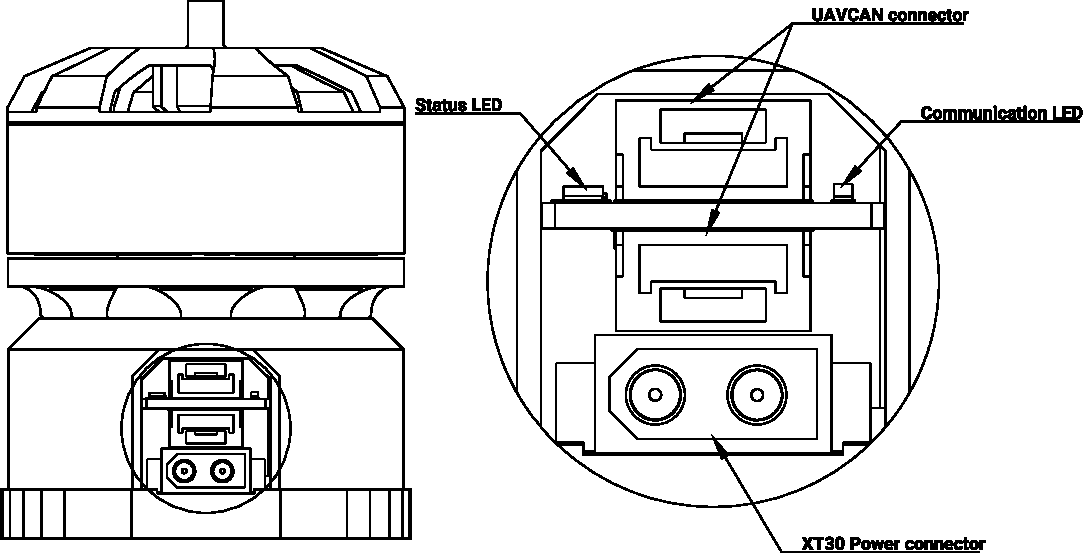
\includegraphics[width=0.8\textwidth]{figures/connectors_leds}}
    \caption{Connectors and LEDs drawing\label{connecotrs}}
\end{figure}

\subsection{Mounting pattern}

All versions of Zubax Sadulli share the same mounting pattern. 
It is specified in the drawing \ref{mounting_pattern} All linear dimensions are in mm.

\begin{figure}[!hbt]
    \centerline{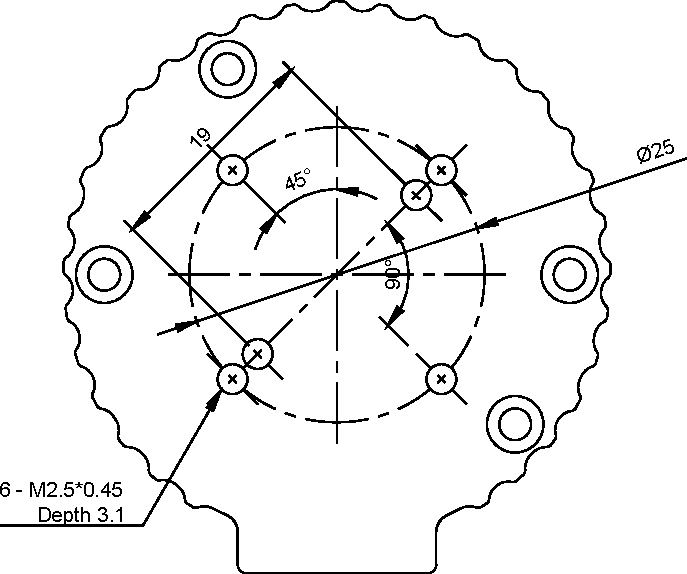
\includegraphics[width=0.7\textwidth]{figures/mounting_pattern}}
    \caption{Mounting pattern\label{mounting_pattern}}
\end{figure}

\newpage

\subsection{Sadulli nudo drawing}
All linear dimensions are in mm.

\begin{figure}[!hbt]
    \centerline{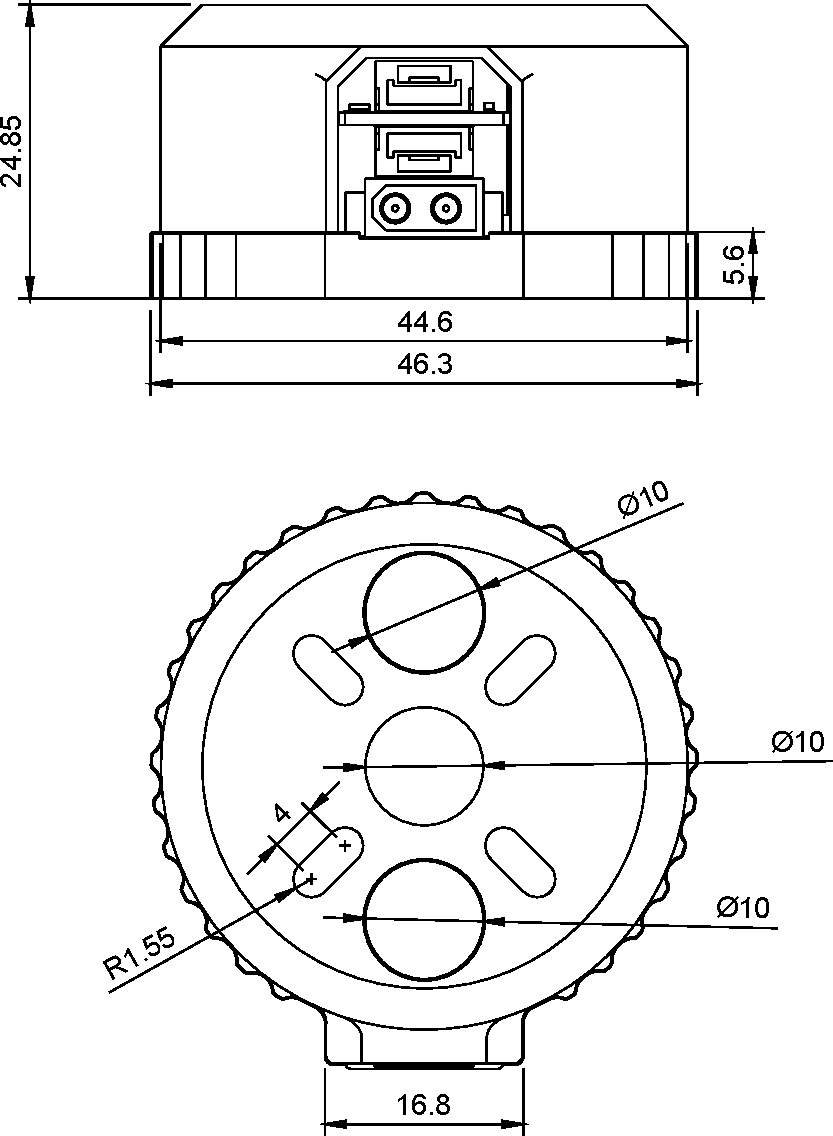
\includegraphics[width=0.8\textwidth]{figures/sadulli_nudo}}
    \caption{Sadulli Nudo drawing\label{Nudo_drawing}}
\end{figure}

\newpage

\subsection{Sadulli Piccino drawing}
All linear dimensions are in mm. Propeller not shown.

\begin{figure}[!hbt]
    \centerline{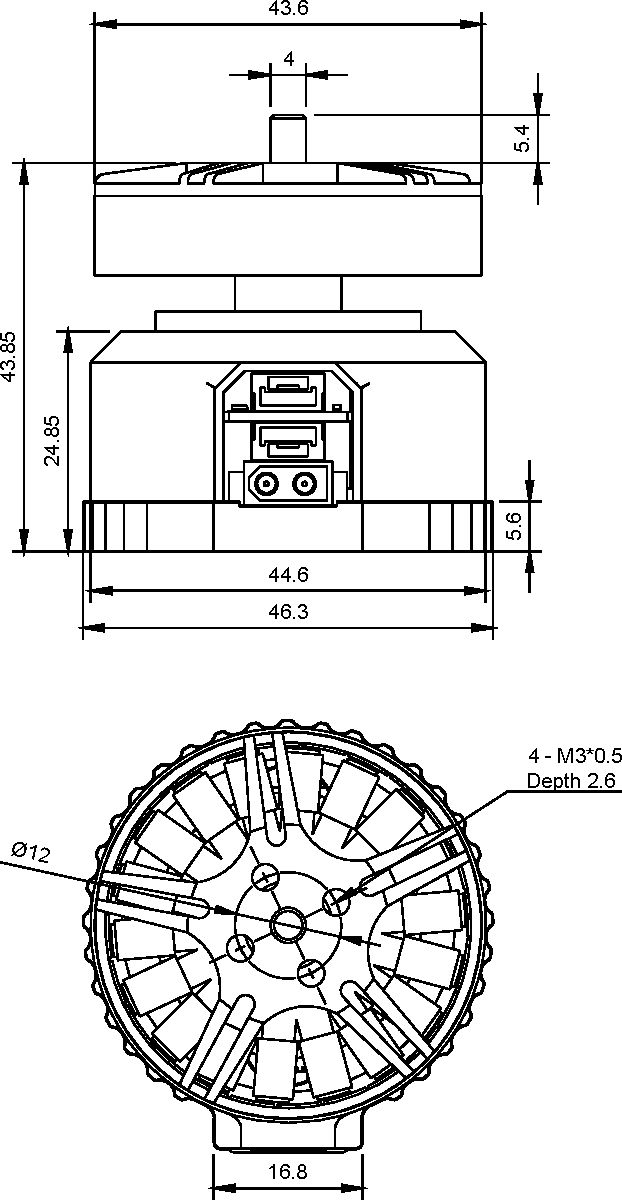
\includegraphics[width=0.6\textwidth]{figures/sadulli_piccino}}
    \caption{Sadulli Piccino drawing\label{Piccino_drawing}}
\end{figure}

\newpage

\subsection{Sadulli Grosso drawing}
All linear dimensions are in mm. Propeller not shown.

\begin{figure}[!hbt]
    \centerline{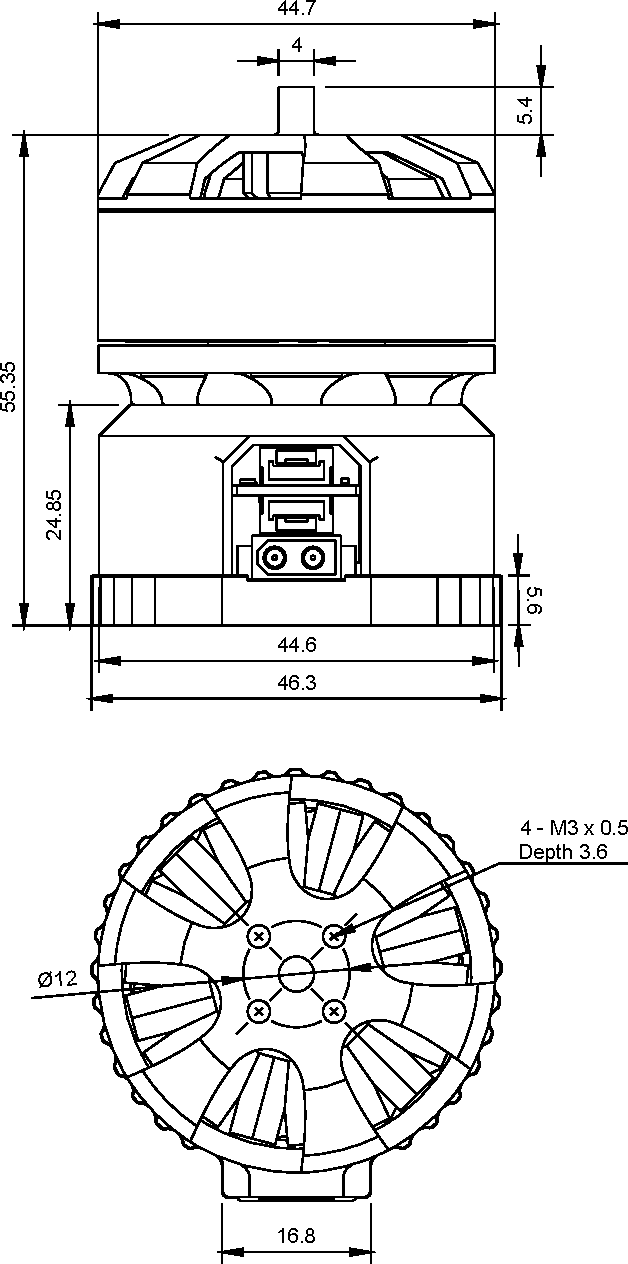
\includegraphics[width=0.6\textwidth]{figures/sadulli_grosso}}
    \caption{Sadulli Grosso drawing\label{Grosso_drawing}}
\end{figure}

\chapter{Indication}

\newcommand{\LEDX}{{\rule{0.4em}{1.0em}}}
\newcommand{\LEDO}{{\rule{0.4em}{0.1em}}}
\newcommand{\ShowColor}[1]{{\color{#1}\rule{2em}{0.8em}}}

Zubax Sadulli is equipped with two separate LED indicators that reflect its status.

\textbf{CAN} green LED indicates data transfer through the CAN bus. 
Blinks once if at least one CAN frame was successfully transmitted or successfully received in the last 25 milliseconds. 
Glows steadily when the intensity of CAN traffic is higher than 40 frames per second.

\textbf{STATUS} RGB LED indicates the status of the firmware. 
The behaviour of the status LED is specified in the table below.

\begin{ZubaxSimpleTable}{Status LED during boot}{|l l X|}
             Color              & Status                              & Description                                      \\
    \ShowColor{yellow} Yellow   & No application to boot              & The firmware has not been flashed to the ESC
                                                                        or FLASH has been damaged.                       \\
    \ShowColor{blue} Blue       & Application upgrade is in progress  &                                                  \\
    \ShowColor{green} Green     & Boot canceled                       & The device firmware has not been properly signed.\\
    \ShowColor{magenta} Magenta & Ready to boot                       & Glows after the device power-up or restart event
                                                                        until the application starts.                    \\
\end{ZubaxSimpleTable}

\begin{ZubaxSimpleTable}{Status LED behavior}{|l X X|}
    LED pattern (step 80 ms)                     & Status                    & Description\\

    {\color{blue}
       \LEDX\LEDO\LEDO\LEDO\LEDO\LEDX}           & Idle, ready to run        & The ESC is ready and waiting for the
                                                                               setpoint.\\
    
    {\color{red}
       \LEDX\LEDO\LEDO\LEDO\LEDO\LEDX\LEDX\LEDX} & Idle, hardware fault      & The power stage is not ready or current
                                                                               is tripped.\\

    {\color{red}
       \LEDX\LEDO\LEDO\LEDO\LEDO\LEDX\LEDO\LEDX\LEDX\LEDX}
                                                 & Idle, hardware test fault & The motor is not connected or there is a
                                                                               short circuit on the output of the
                                                                               ESC.\\

    {\color{red}
       \LEDX\LEDO\LEDO\LEDO\LEDO\LEDX\LEDO\LEDX\LEDO\LEDX\LEDO\LEDX\LEDO\LEDX\LEDO\LEDX\LEDO\LEDX\LEDX\LEDX\LEDO\LEDX
       \LEDX\LEDX}                          & Idle, invalid motor parameters & Some motor parameters are not properly
                                                                               initialized or the motor identification
                                                                               hasn't been performed.\\
\end{ZubaxSimpleTable}


\chapter{Mechanical characteristics}

\begin{ZubaxSimpleTable}{Mechanical characteristics}{| l | c | c | c | X | c |}
    Parameter       & Grosso  & Piccino  & Nudo  & Note                                & Unit \\
    Mass            & 228     & 128      & 62    & Cables and propellers not included     & g \\
    IP Protection   & 54      & 54       & 54    & Liquid damage protection is achieved 
                                                   by conformal \mbox{coating} of the PCB &   \\
\end{ZubaxSimpleTable}

The drawing \ref{fig:characteristics_connectors_placement} documents the placement of connectors and status LEDs on all variants of Zubax Sadulli.

\begin{figure}[!hbt]
    \centerline{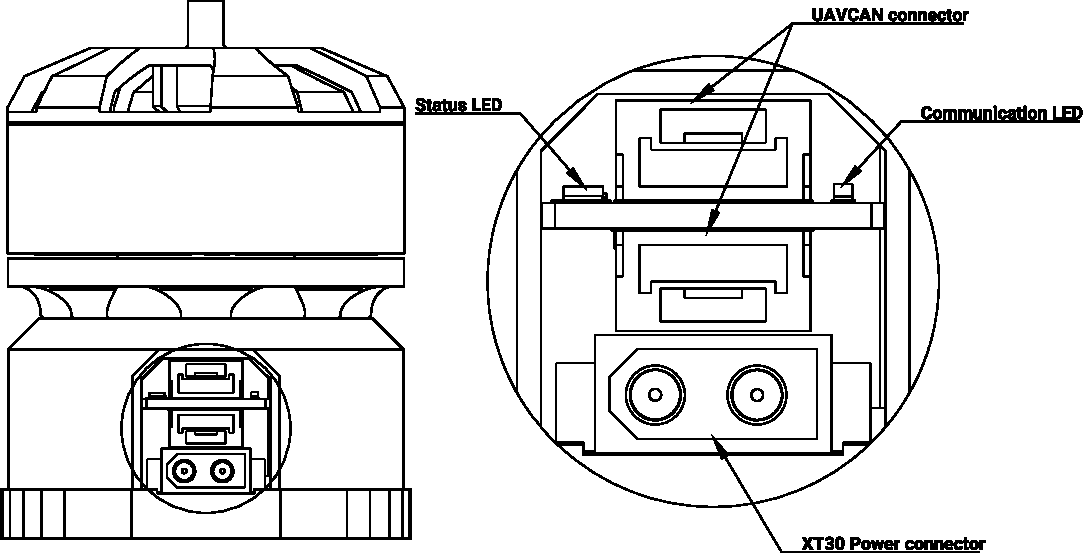
\includegraphics[width=0.8\textwidth]{figures/connectors_leds}}
    \caption{Connectors and LEDs drawing\label{fig:characteristics_connectors_placement}}
\end{figure}

\section{Mounting pattern}

All versions of Zubax Sadulli share the same mounting pattern. 
It is specified in the drawing \ref{fig:characteristics_mounting_pattern}. All linear dimensions are in mm.

\begin{figure}[!hbt]
    \centerline{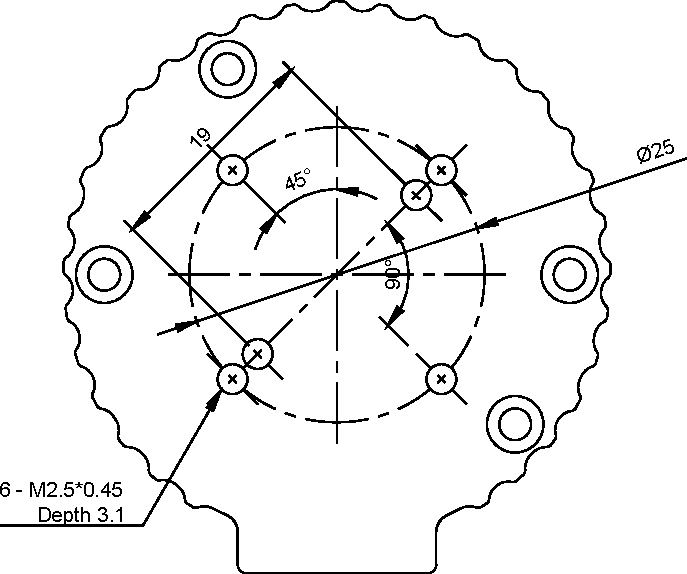
\includegraphics[width=0.5\textwidth]{figures/mounting_pattern}}
    \caption{Mounting pattern\label{fig:characteristics_mounting_pattern}}
\end{figure}

\newpage

\section{Sadulli nudo drawing}
All linear dimensions are in mm.

\begin{figure}[!hbt]
    \centerline{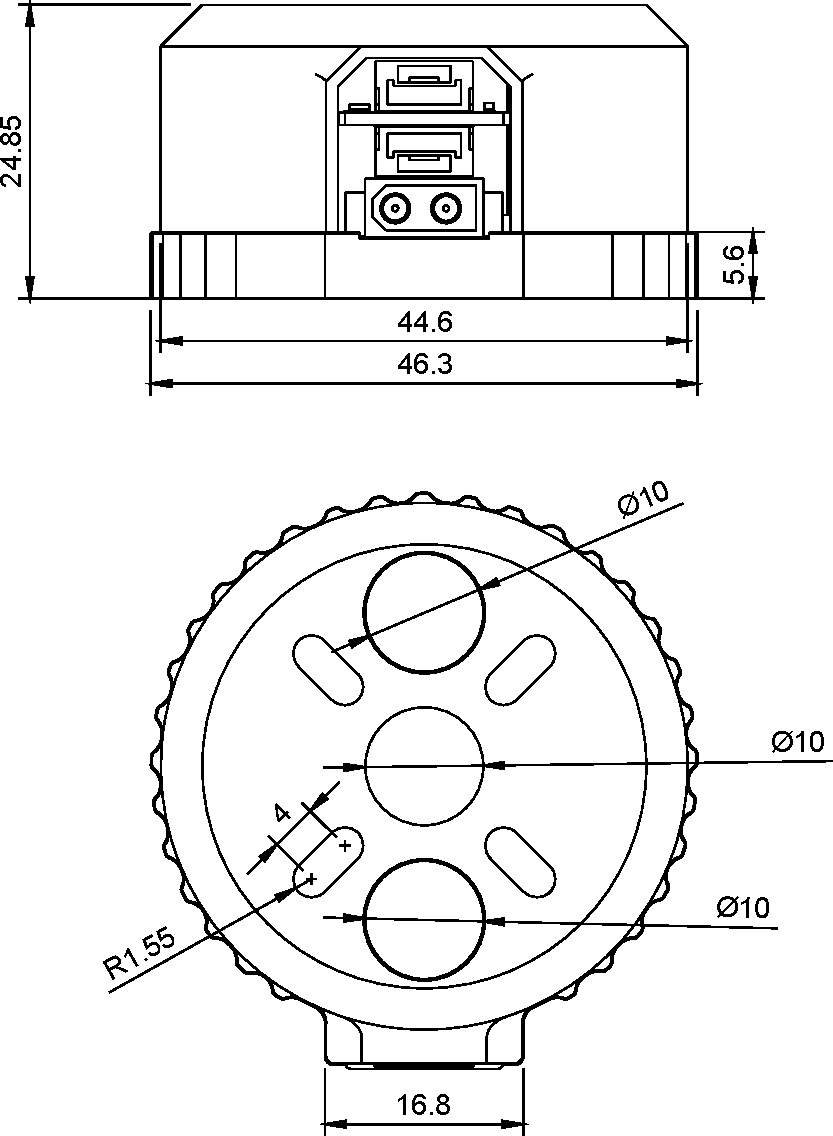
\includegraphics[width=0.6\textwidth]{figures/sadulli_nudo}}
    \caption{Sadulli Nudo drawing}
\end{figure}

\newpage

\section{Sadulli Piccino drawing}
All linear dimensions are in mm. Propeller not shown.

\begin{figure}[!hbt]
    \centerline{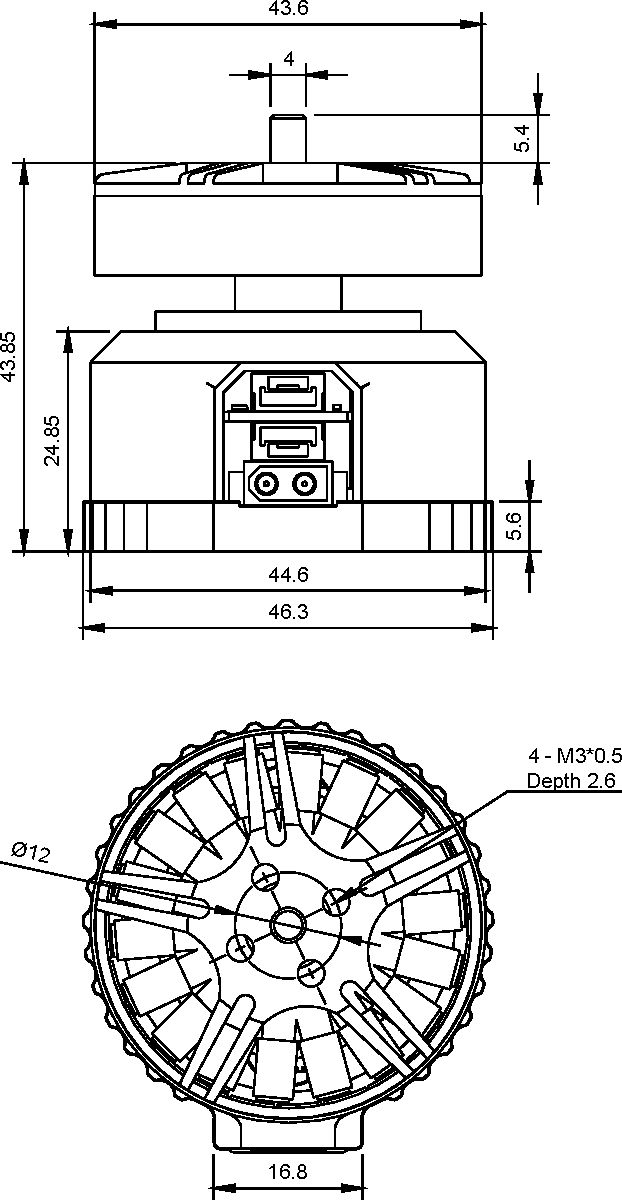
\includegraphics[width=0.6\textwidth]{figures/sadulli_piccino}}
    \caption{Sadulli Piccino drawing}
\end{figure}

\newpage

\section{Sadulli Grosso drawing}
All linear dimensions are in mm. Propeller not shown.

\begin{figure}[!hbt]
    \centerline{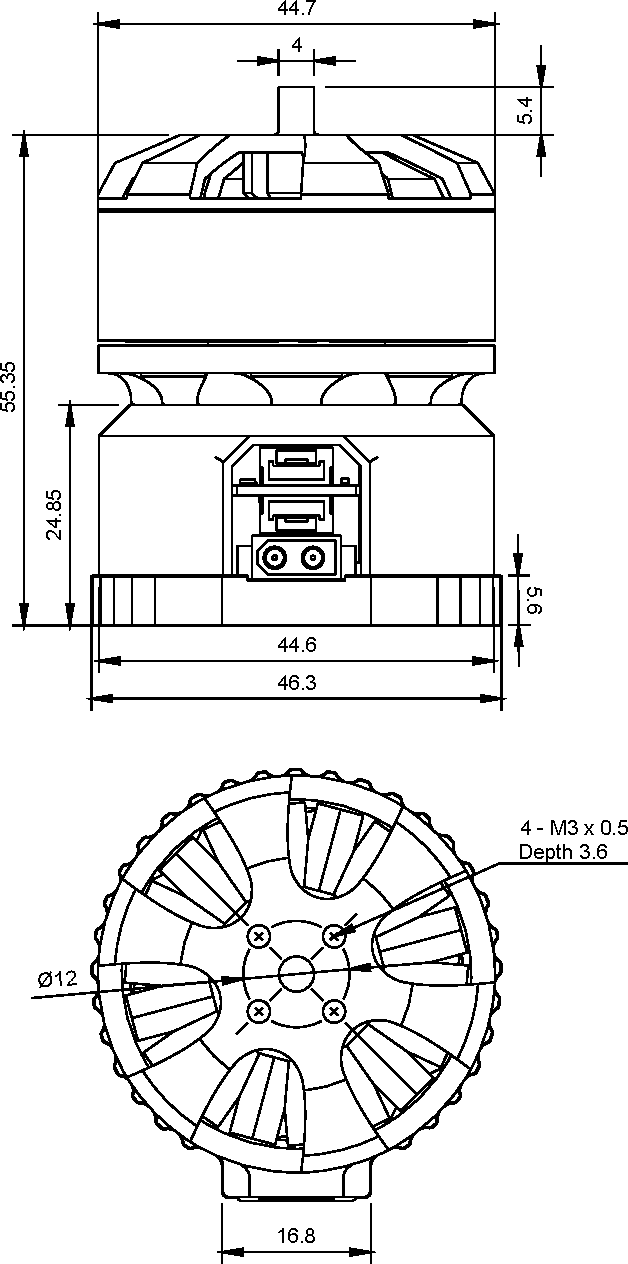
\includegraphics[width=0.6\textwidth]{figures/sadulli_grosso}}
    \caption{Sadulli Grosso drawing}
\end{figure}

\chapter{Thrust characteristics}

Graphs below present empirical data on the thrust produced by Sadulli Piccino and Sadulli Grosso. 
All data collected at normal conditions: standard atmospheric pressure (100 kPa) and normal temperature (25\degree{}C) at MSL.

\begin{ZubaxTableWrapper}{Propeller characteristics}
    \begin{ZubaxWrappedTable}{| X | X | X | X |}
    Parameter           & Sadulli Piccino   & Sadulli Grosso & Unit \\
    Propeller diameter  & 15                & 17             & inch \\
    Propeller pitch     & 5.5               & 6.2            & inch \\
\end{ZubaxWrappedTable}
\end{ZubaxTableWrapper}

\begin{figure}[!hbt]
    \centerline{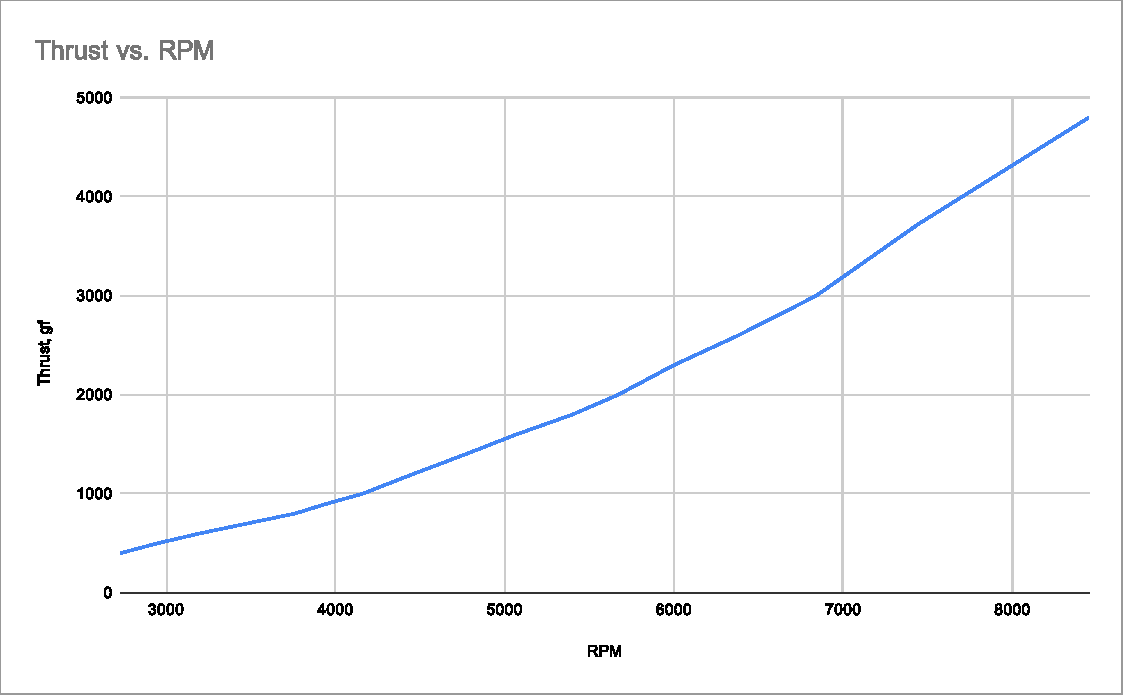
\includegraphics[width=0.75\textwidth]{figures/propeller_1555.pdf}}
    \caption{Sadulli Piccino propeller thrust vs. RPM\label{Piccino_thrust}}
\end{figure}

\begin{figure}[!hbt]
    \centerline{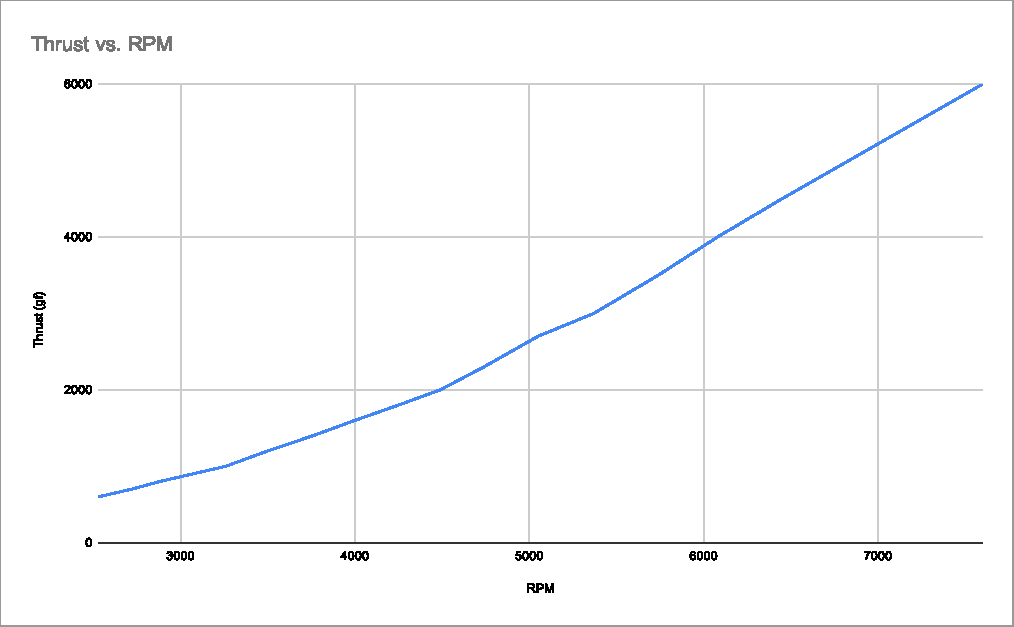
\includegraphics[width=0.75\textwidth]{figures/propeller_1762.pdf}}
    \caption{Sadulli Grosso propeller thrust vs. RPM\label{Grosso_thrust}}
\end{figure}

\newpage

\section{Thrust-power ratio}

In the realm of constant pitch propeller drives, there is a tendency for thrust efficiency reduction 
with the increase of propeller RPM. This means that although maximum thrust is limited by propeller material 
and motor and controller power limitations and may reach relatively high values,  
it may be beneficial not to use the drive at its maximum thrust levels and stay at relatively low RPM 
where the efficiency is higher. The specific efficiency level proposed for optimum operation is 10 gf/W. 
Aircraft designer should keep that in mind and select the propulsion system accordingly.

\begin{figure}[!hbt]
    \centerline{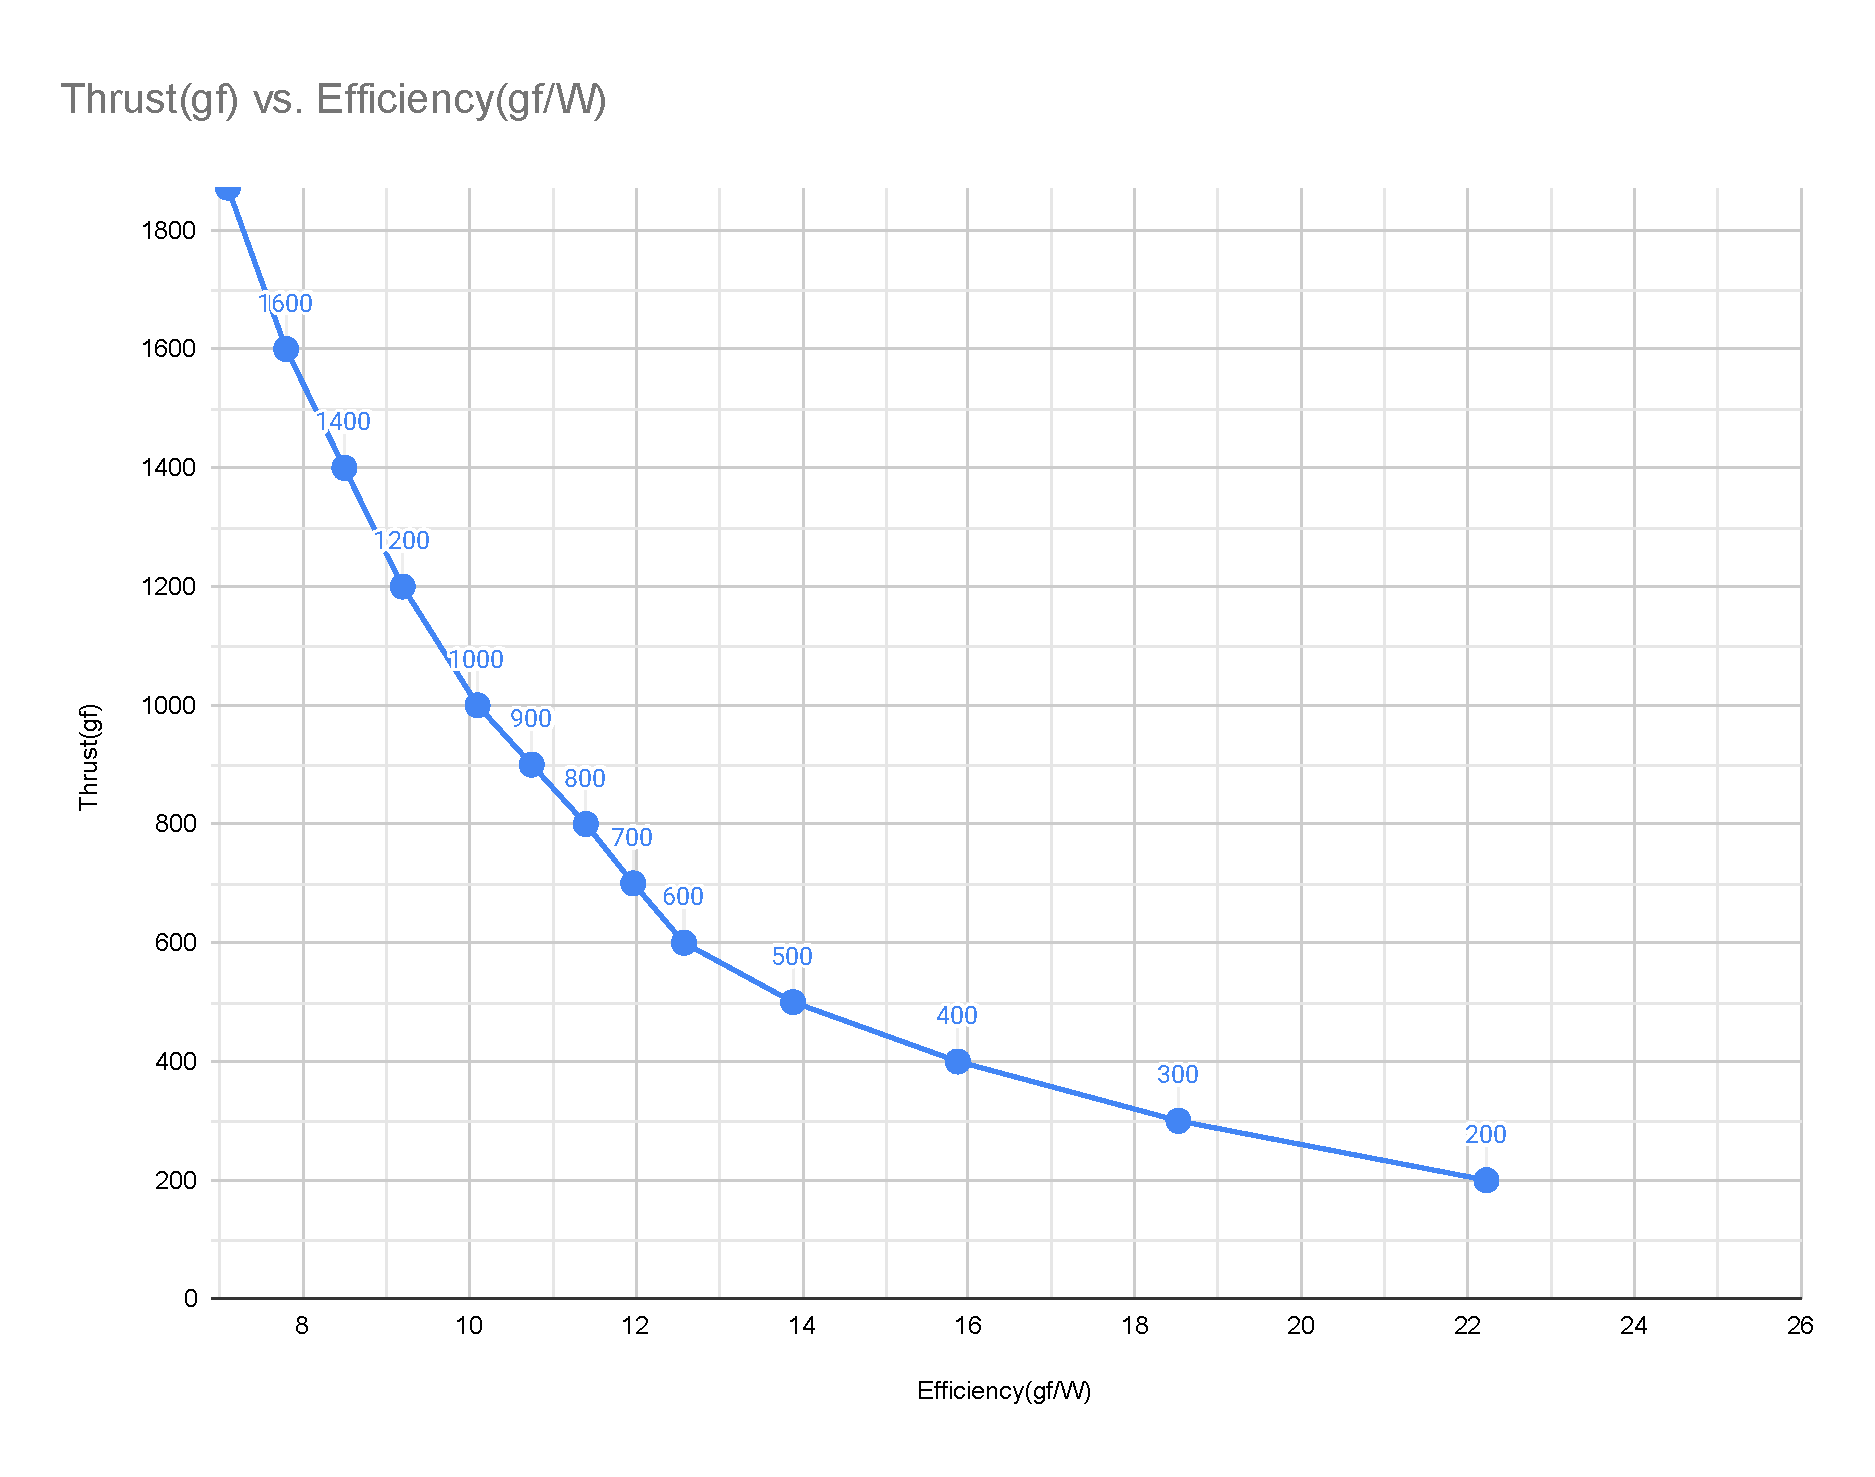
\includegraphics[width=0.7\textwidth]{figures/thrust-efficiency_piccino.pdf}}
    \caption{Sadulli Piccino Thrust vs. Efficiency\label{Piccino_thrust_vs_efficiency}}
\end{figure}

\begin{figure}[!hbt]
    \centerline{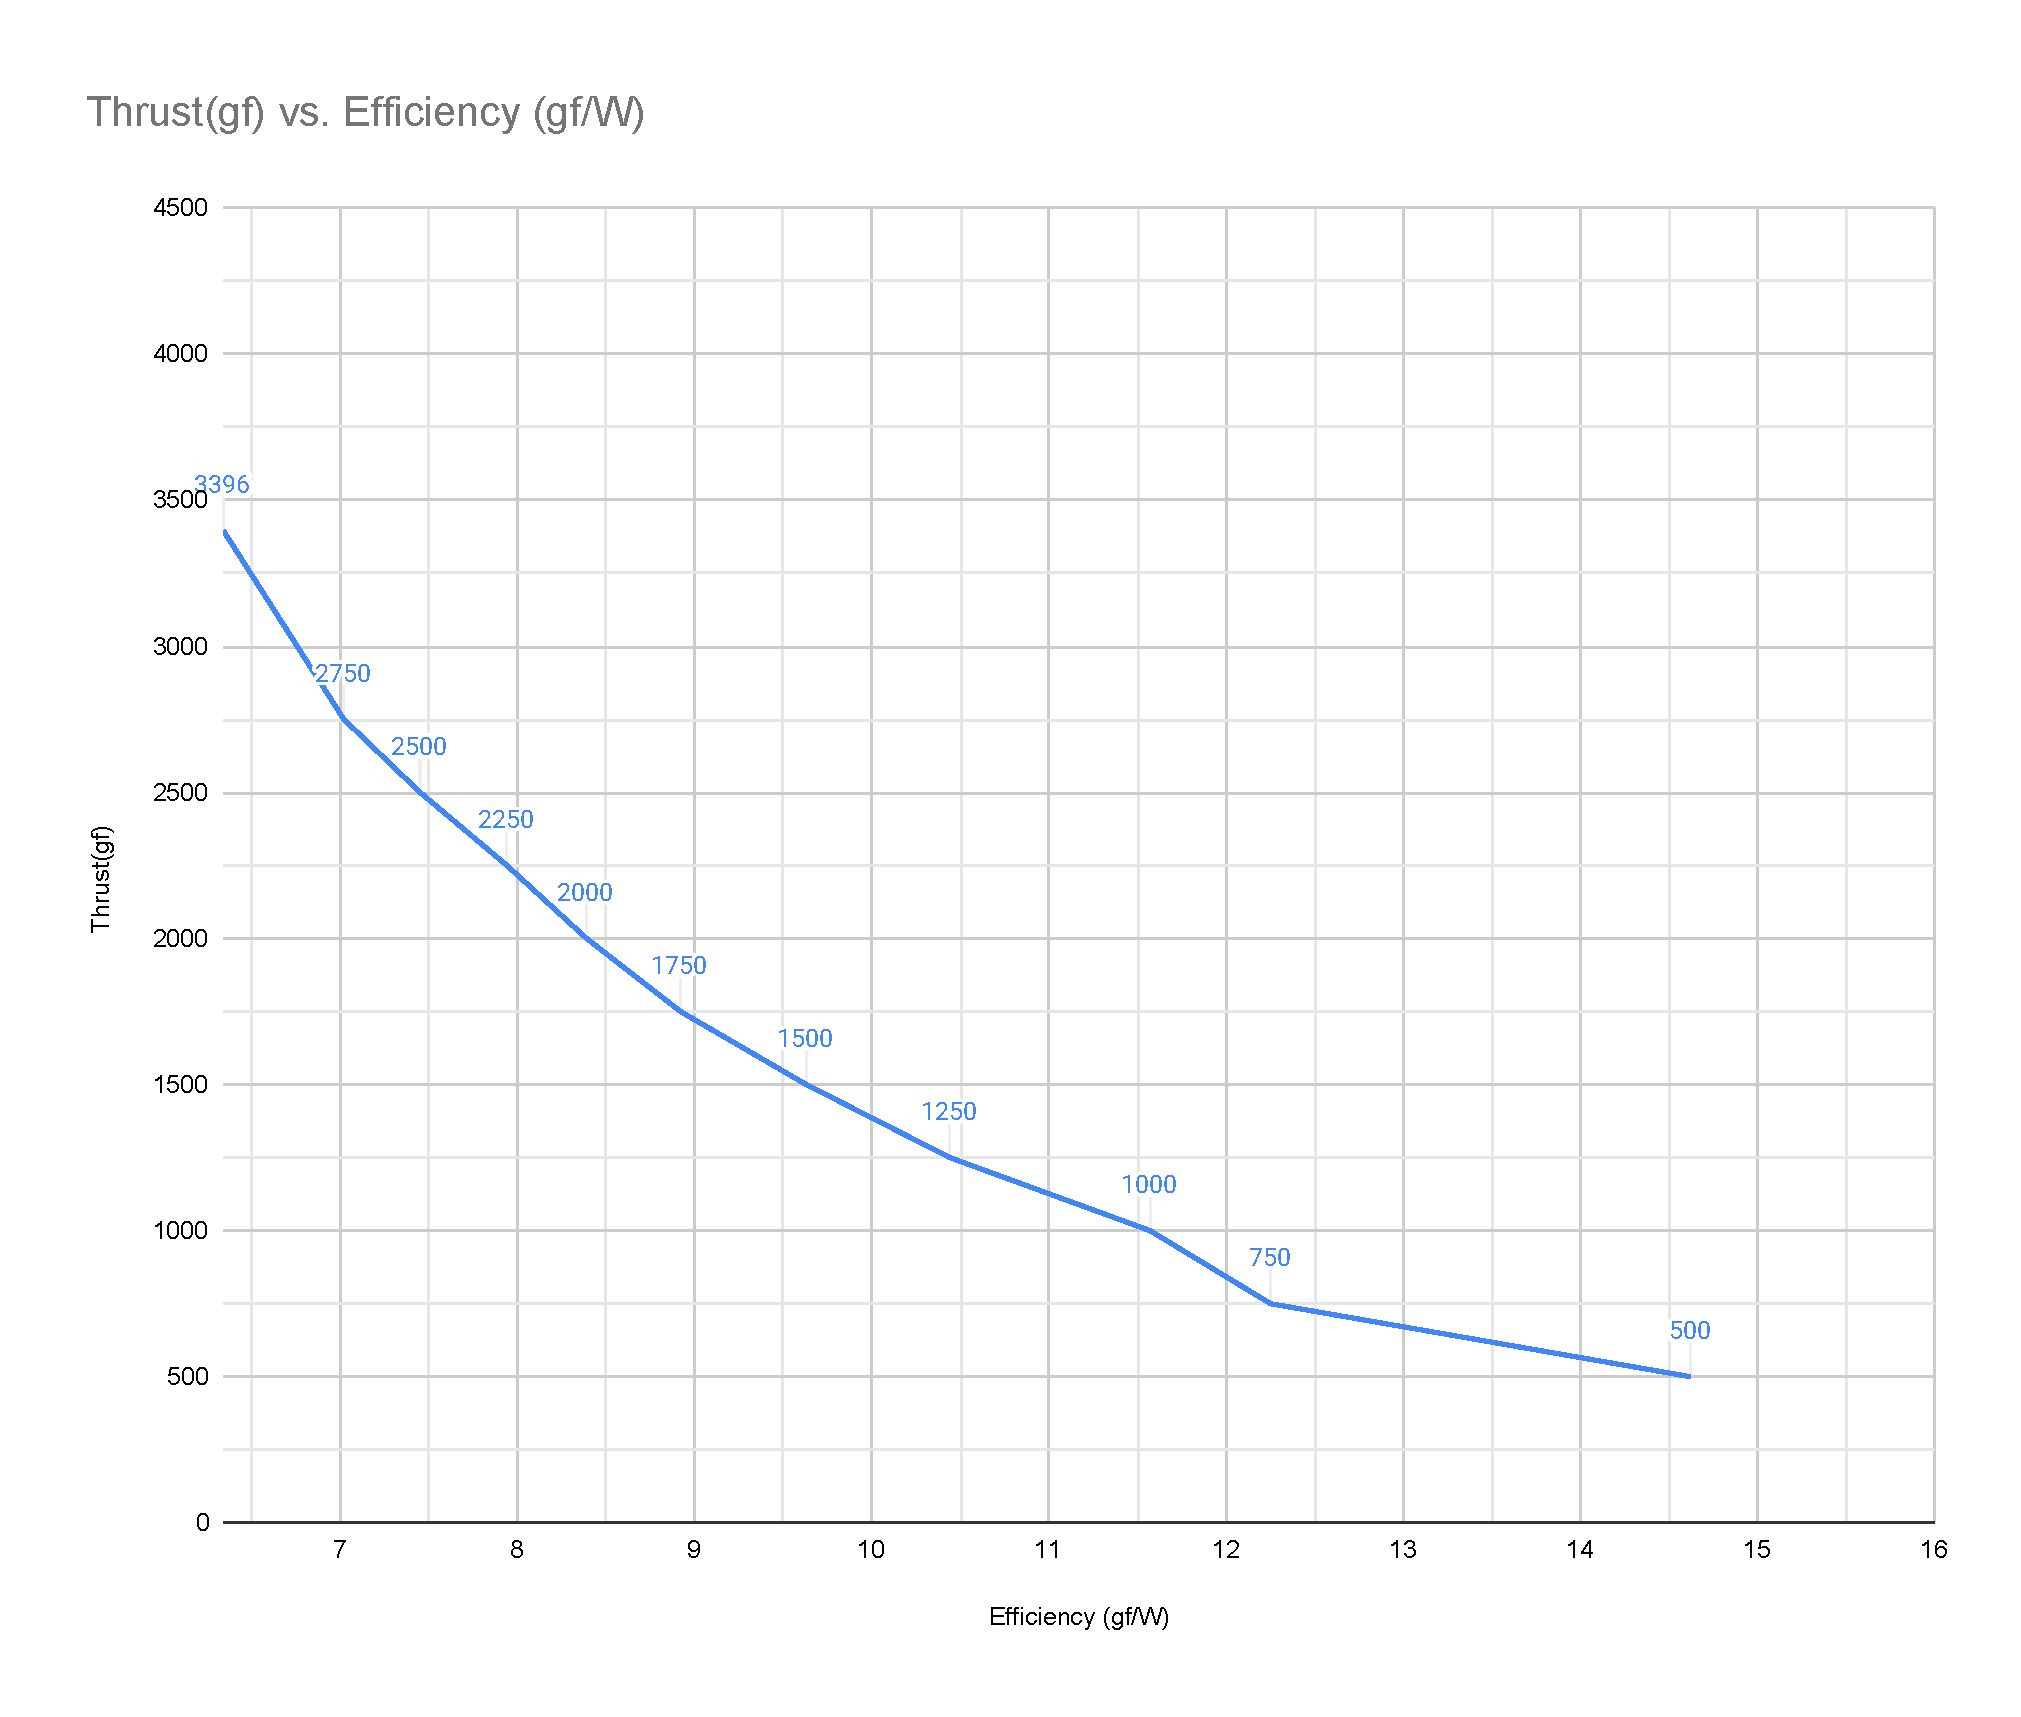
\includegraphics[width=0.7\textwidth]{figures/thrust-efficiency_grosso.pdf}}
    \caption{Sadulli Grosso Thrust vs. Efficiency\label{Grosso_thrust_vs_efficiency}}
\end{figure}


\end{document}
